\chapter*{Scopo del documento}
\addcontentsline{toc}{chapter}{Scopo del documento}
Il presente documento riporta la definizione dell’architettura del progetto "Sistema monitoraggio ambientale" usando il diagramma delle classi in Unified Modeling Language (UML). Viene inoltre introdotto il linguaggio Object Constraint Language (OCL) per esprimere vincoli che altrimenti non sarebbe possibili esporre mediante UML in modo formale e preciso.
Per rappresentare l'architettura del sistema viene utilizzato il diagramma delle classi in linguaggio UML che dovranno essere implementate a livello di codice; viene inoltre spiegata la logica dietro il corretto funzionamento del sistema.

\chapter{Diagramma delle classi}

Nel presente capitolo vengono presentate le classi previste nell’ambito del progetto "Sistema di monitoraggio ambientale". Ogni attore e ogni sistema esterno presenti nel diagramma di contesto diventano una o più classi. 

\section{Autenticatore}
Nel nostro sistema, come è possibile osservare nel component diagram, è presente un elemento incaricato di gestire l'autenticazione di un amministratore. Questa funzionalità è stata modellata con la classe \texttt{Autenticatore}. L'autenticazione viene effettuata controllando i dati inseriti dall'utente attraverso la funzione \\ \texttt{verifica\_credenziali(String email,String password)}. Questa funzione quindi chiamerà al suo interno  \texttt{Interfaccia\_database.get\_password(String email)} e confronterà il suo valore di ritorno con quello inserito dall'utente. Di seguito la classe con i suoi attributi e metodi.

\begin{figure}[ht]
    \centering
    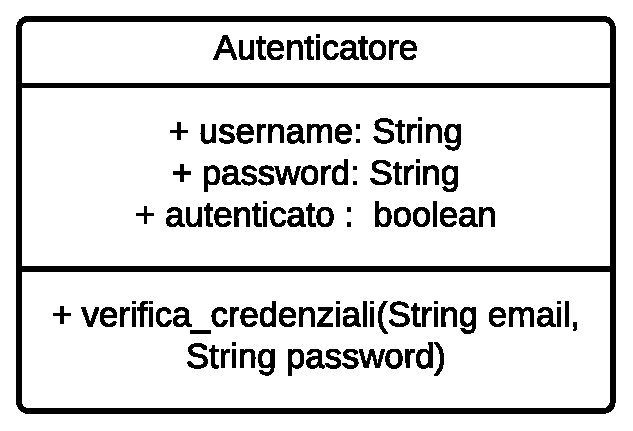
\includegraphics[scale=0.4]{Img/ClassAutenticatore.eps}
\end{figure}

\section{Visualizzatore menù principale}
Analizzando il diagramma di contesto del sistema si nota la presenza di due attori: "Utente non autenticato" e "Amministratore". L'utente non autenticato è in grado di ricevere delle notifiche di allarme in caso di allerta ambientale e può ottenere informazioni sulla flora e la fauna. L'amministratore, invece, è in grado di effettuare funzionalità più complesse, ossia ottenere lo storico di animali specifici in un determinato lasso di tempo, ottenere statistiche sulla valutazione dei rischi e gestire il parco. 

Il componente "visualizzatore menù principale" presentato nel diagramma dei componenti viene implementato utilizzando una classe con il medesimo nome. Esso permette all'utente di svolgere le attività secondo il livello di accesso che esso possiede secondo il principio del "Need to Know". Il metodo \texttt{aggiorna\_pagina()} permette all'applicazione di fornire la pagina richiesta comunicando con \texttt{Interfaccia\_database} ed il \texttt{Generatore\_istogrammi}, secondo il livello di accesso possesso dall'utente.

Le pagine vengono fornite creando un'istanza della classe \texttt{Pagina} in base alla richiesta dell'utente. Per esempio, nel caso in cui venga richiesto una pagina contenente la descrizione di una determinata specie, essa conterrà immagini di animali di quella specie, la loro descrizione e le posizioni in tempo reale degli animali sulla mappa del parco.

\begin{figure}[ht]
    \centering
    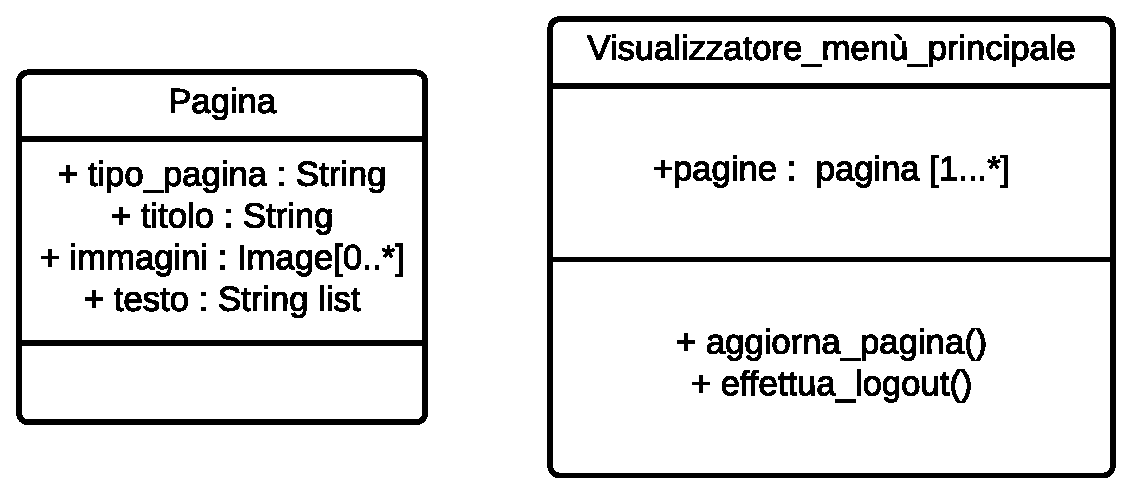
\includegraphics[scale=0.4]{Img/ClassMenu.eps}
\end{figure}

\newpage
\section{Interfaccia Database}
Il componente "Interfaccia Base di Dati" è necessario per il corretto funzionamento del sistema in quanto gli permette di dialogare con il database esterno. La classe \texttt{Interfaccia\_database} implementa tali funzionalità e permette ai componenti interni di ottenere i dati richiesti. Di seguito viene esposta la classe con i suoi attributi ed i suoi metodi. 

\begin{figure}[ht]
    \centering
    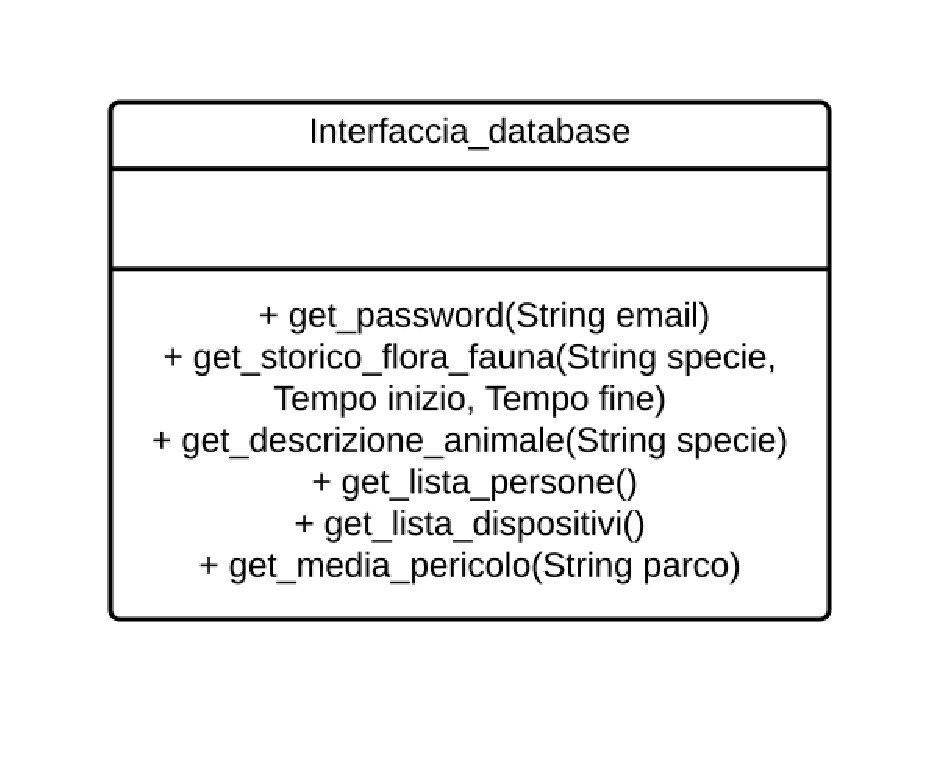
\includegraphics[scale=0.35]{Img/ClassDataBase.eps}
\end{figure}

\section{Generatore Istogrammi}
Analizzando il componente "Generatore istogrammi", necessario per creare i grafici sullo storico di un animale, abbiamo identificato 3 classi \texttt{Generatore\_istogramma}, \texttt{Istogramma}, \texttt{Tempo} con attributi e funzioni specifici.

In particolare la classe \texttt{Generatore\_istogramma} è in grado di creare un'immagine partendo da un dato di tipo \texttt{Istogramma}, il quale racchiude tutti i dati necessari richiesti dall'utente.

\begin{figure}[ht]
    \centering
    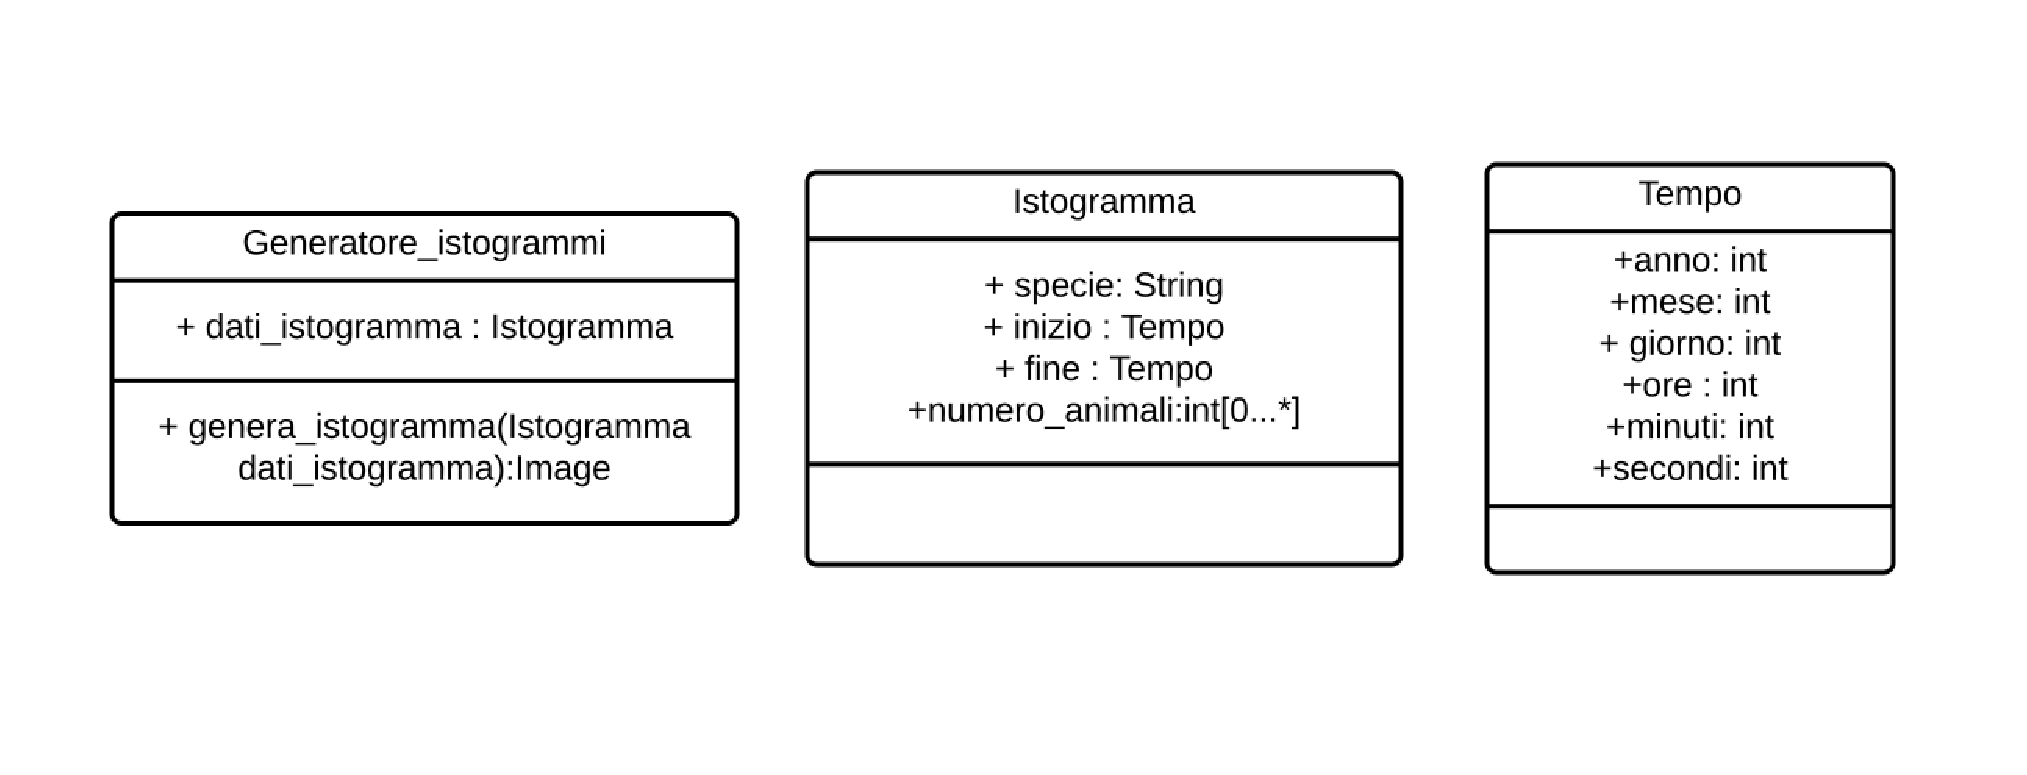
\includegraphics[scale=0.4]{Img/ClassIstogramma.eps}
\end{figure}

\section{Gestione sensori GPS}

Come si può vedere nel diagramma di contesto, il sistema dovrà comunicare con il Sistema GPS.
Questo è stato reso possibile realizzando la classe \texttt{Sensore\_GPS} e la classe \texttt{gestione\_sensori\_GPS}: 
\begin{itemize}
    \item la prima è caratterizzata da degli attributi che identificano univocamente a quale animale è assegnato, mentre le funzioni permettono principalmente di monitorare la posizione di esso. Nel caso in cui un animale esca dal suo parco di appartenenza, il sensore è in grado di capire che si trova fuori dalla zona a lui assegnata, e l'attributo \texttt{contenimento\_sensore} cambia valore in false. Questa informazione verrà poi percepita da un'istanza della classe \texttt{interfaccia\_notifiche} per inviare le dovute segnalazioni.
    \item la seconda invece memorizza tutti i sensori e il numero totale di essi, implementando anche metodi per aggiungere o rimuovere unità dal sistema.
\end{itemize}

\begin{figure}[ht]
    \centering
    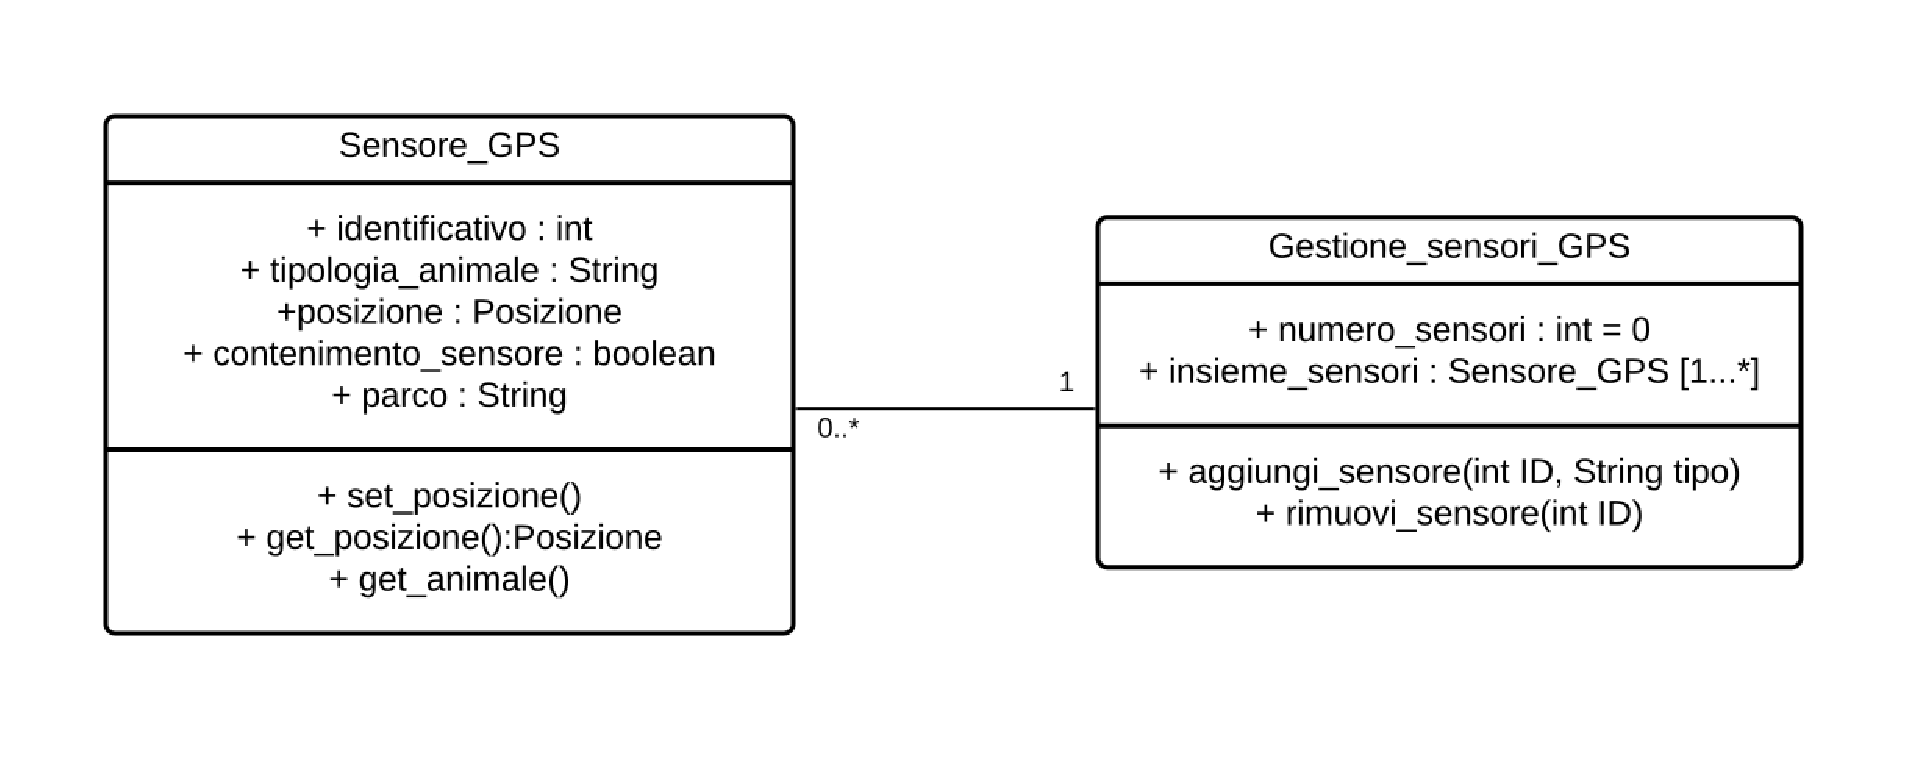
\includegraphics[scale=0.35]{Img/ClassSensoriGPS.eps}
\end{figure}

\newpage
\section{Gestione sensori ambientali}
Nel diagramma di contesto sono presenti due sistemi esterni chiamati Sensori e Sistema calcolo probabilistico.
Le entità di cui sopra sono state modellate in questo class diagram attraverso le classi \texttt{Sensore ambientale} e \texttt{Interfaccia calcolo probabilistico}.
Gli attributi appartenenti alla classe \texttt{Sensore\_ambientale} sono utili per identificarli univocamente all'interno di un parco e per descriverne la loro natura (per descrivere il loro compito all'interno del sistema). Infatti è stato creato il nuovo tipo \texttt{Tipo\_sensore} che descrive se il sensore è designato ad acquisire informazioni su allagamento, siccità, incendio, termine delle risorse idriche o meteo. Inoltre questa classe permette di registrare i valori grezzi e raffinati del pericolo della rispettiva categoria.
La classe Interfaccia calcolo probabilistico invece permette di memorizzare la totalità dei sensori nella \texttt{lista sensori\_amb} e anche la media delle percentuali di pericolo per ogni categoria di pericolo. Parlando dei metodi invece è possibile notare che \texttt{elabora\_dati(Sensore\_ambientale sensore\_ambientale)} prende in input un sensore e restituisce un intero che andrà a popolare l'attributo \texttt{pericolo\_attuale} di quel sensore. Invece la funzione \texttt{calcola\_media(Sensore\_ambientale[] sensori\_amb, Tipo\_sensore tipo\_sensore)} prende in input l'array di tutti di sensori e il tipo sensore del quale fare la media con l'obiettivo di popolare l'array delle medie.

\begin{figure}[ht]
    \centering
    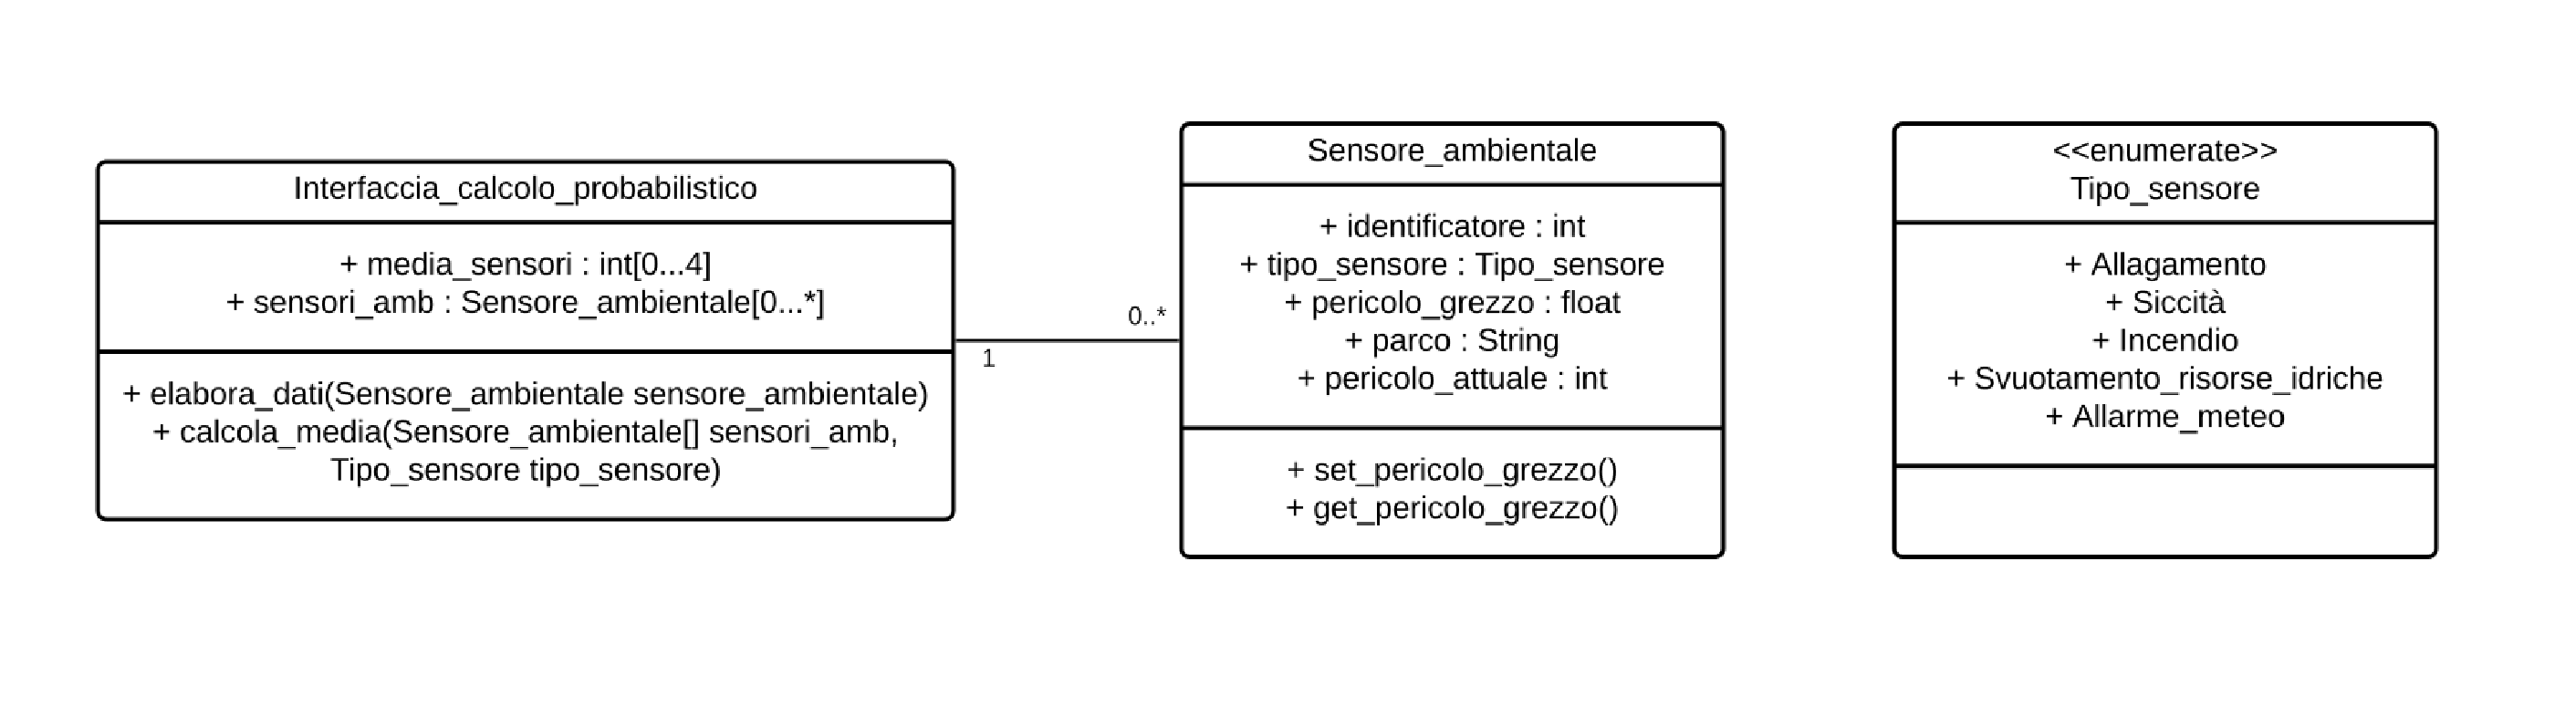
\includegraphics[scale=0.36]{Img/ClassCalcoloProbabilità.eps}
\end{figure}


\section{Interfaccia notifiche}
Questa classe è stata modellata per interfacciarsi al Sistema invio mail/notifiche. In questo progetto abbiamo deciso di implementare un singolo metodo che al suo interno chiamerà le funzioni \\ \texttt{Interfaccia\_database.get\_lista\_persone()} e \texttt{Interfaccia\_database.get\_lista\_dispositivi()} per sapere a quali dispositivi inviare la notifica e a quali mail inviare le segnalazioni. Inoltre, chiamando la funzione \texttt{Interfaccia\_database.get\_media\_pericolo(String parco)}, il sistema sarà in grado di capire il livello di pericolo (vedi documenti precedenti) sapendo le percentuali restituite dalla funzione appena chiamata.

\begin{figure}[ht]
    \centering
    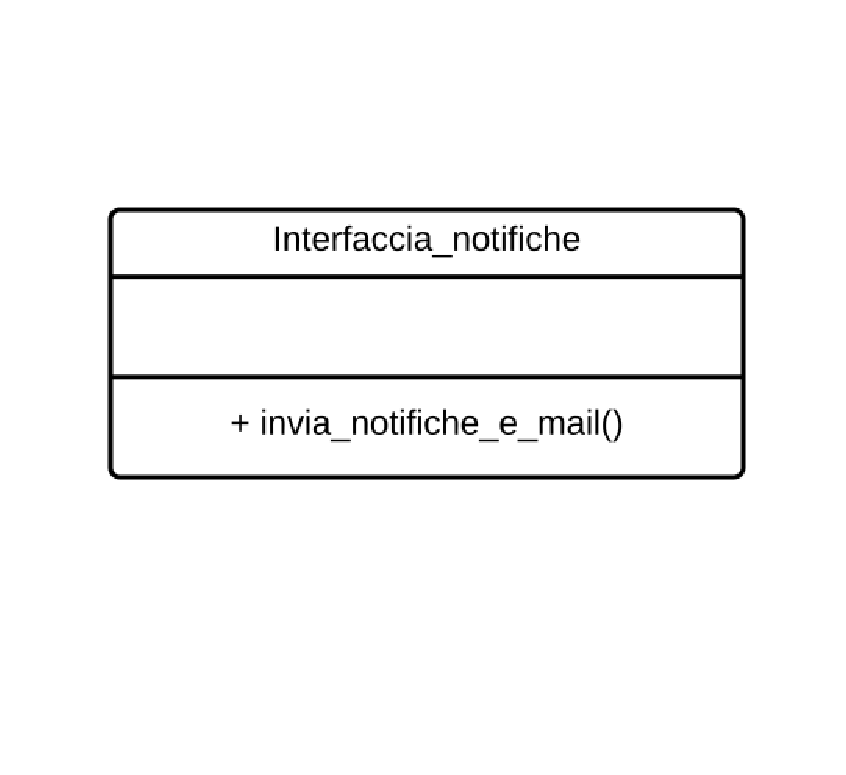
\includegraphics[scale=0.3]{Img/ClassNotifiche.eps}
\end{figure}

\newpage
\section{Diagramma delle classi complessivo}

\begin{figure}[ht]
    \centering
    \includegraphics[scale=0.32]{Img/ClassDiagram.eps}
\end{figure}